% Szglab4
% ===========================================================================
%
\chapter{Prototípus koncepciója}

\thispagestyle{fancy}

\setcounter{section}{-1}
\section{Módosítások a specifikációban}

\subsection{Ragacs kopása}
\textbf{A ragacs eltűnik a pályáról, miután négy robot ráugrott (elkopik).}\newline
A Sticky osztályban létrehozunk egy változót, ami nyilvántartja, hogy hányan ugrottak rá. Ezt a változót az osztály visit(Robot element) metódusa fogja menedzselni.

\subsection{Olaj felszáradása}
\textbf{Egy meghatározott idő letelte után az olajfolt eltűnik a pályáról (felszárad).}\newline
Az Oil osztályban létrehozunk egy változót, ami nyilvántartja a hátralévő idejét. A hátralévő időt úgy menedzseli, hogy az osztály implementálja a HeartBeatListener interfészt és az onTick(long deltaTime) metódusában levonja az eltelt időt.

\subsection{Robotok ütközése}
\textbf{A robotok képesek ütközni, ha azonos helyre érkeznek ugrásuk végén. Ilyenkor a gyorsabb robot összetöri (megsemmisíti) a lassabbat, és kettejük átlagsebességével halad tovább (vektorátlag!).}\newline
A Field onEnter(Agent agent) metódusában, ha a Field-en éppen van egy másik Agent is, akkor meghívjuk a Fielden az éppen rajtalévő Agent collide(Agent agent) metódusát. A collide-ban a vesztesre meghívjuk az agent.accept(new KillExecute) metódust.

\clearpage

\subsection{Osztálydiagram módosítások}
\begin{figure}[h]
	\begin{center}
		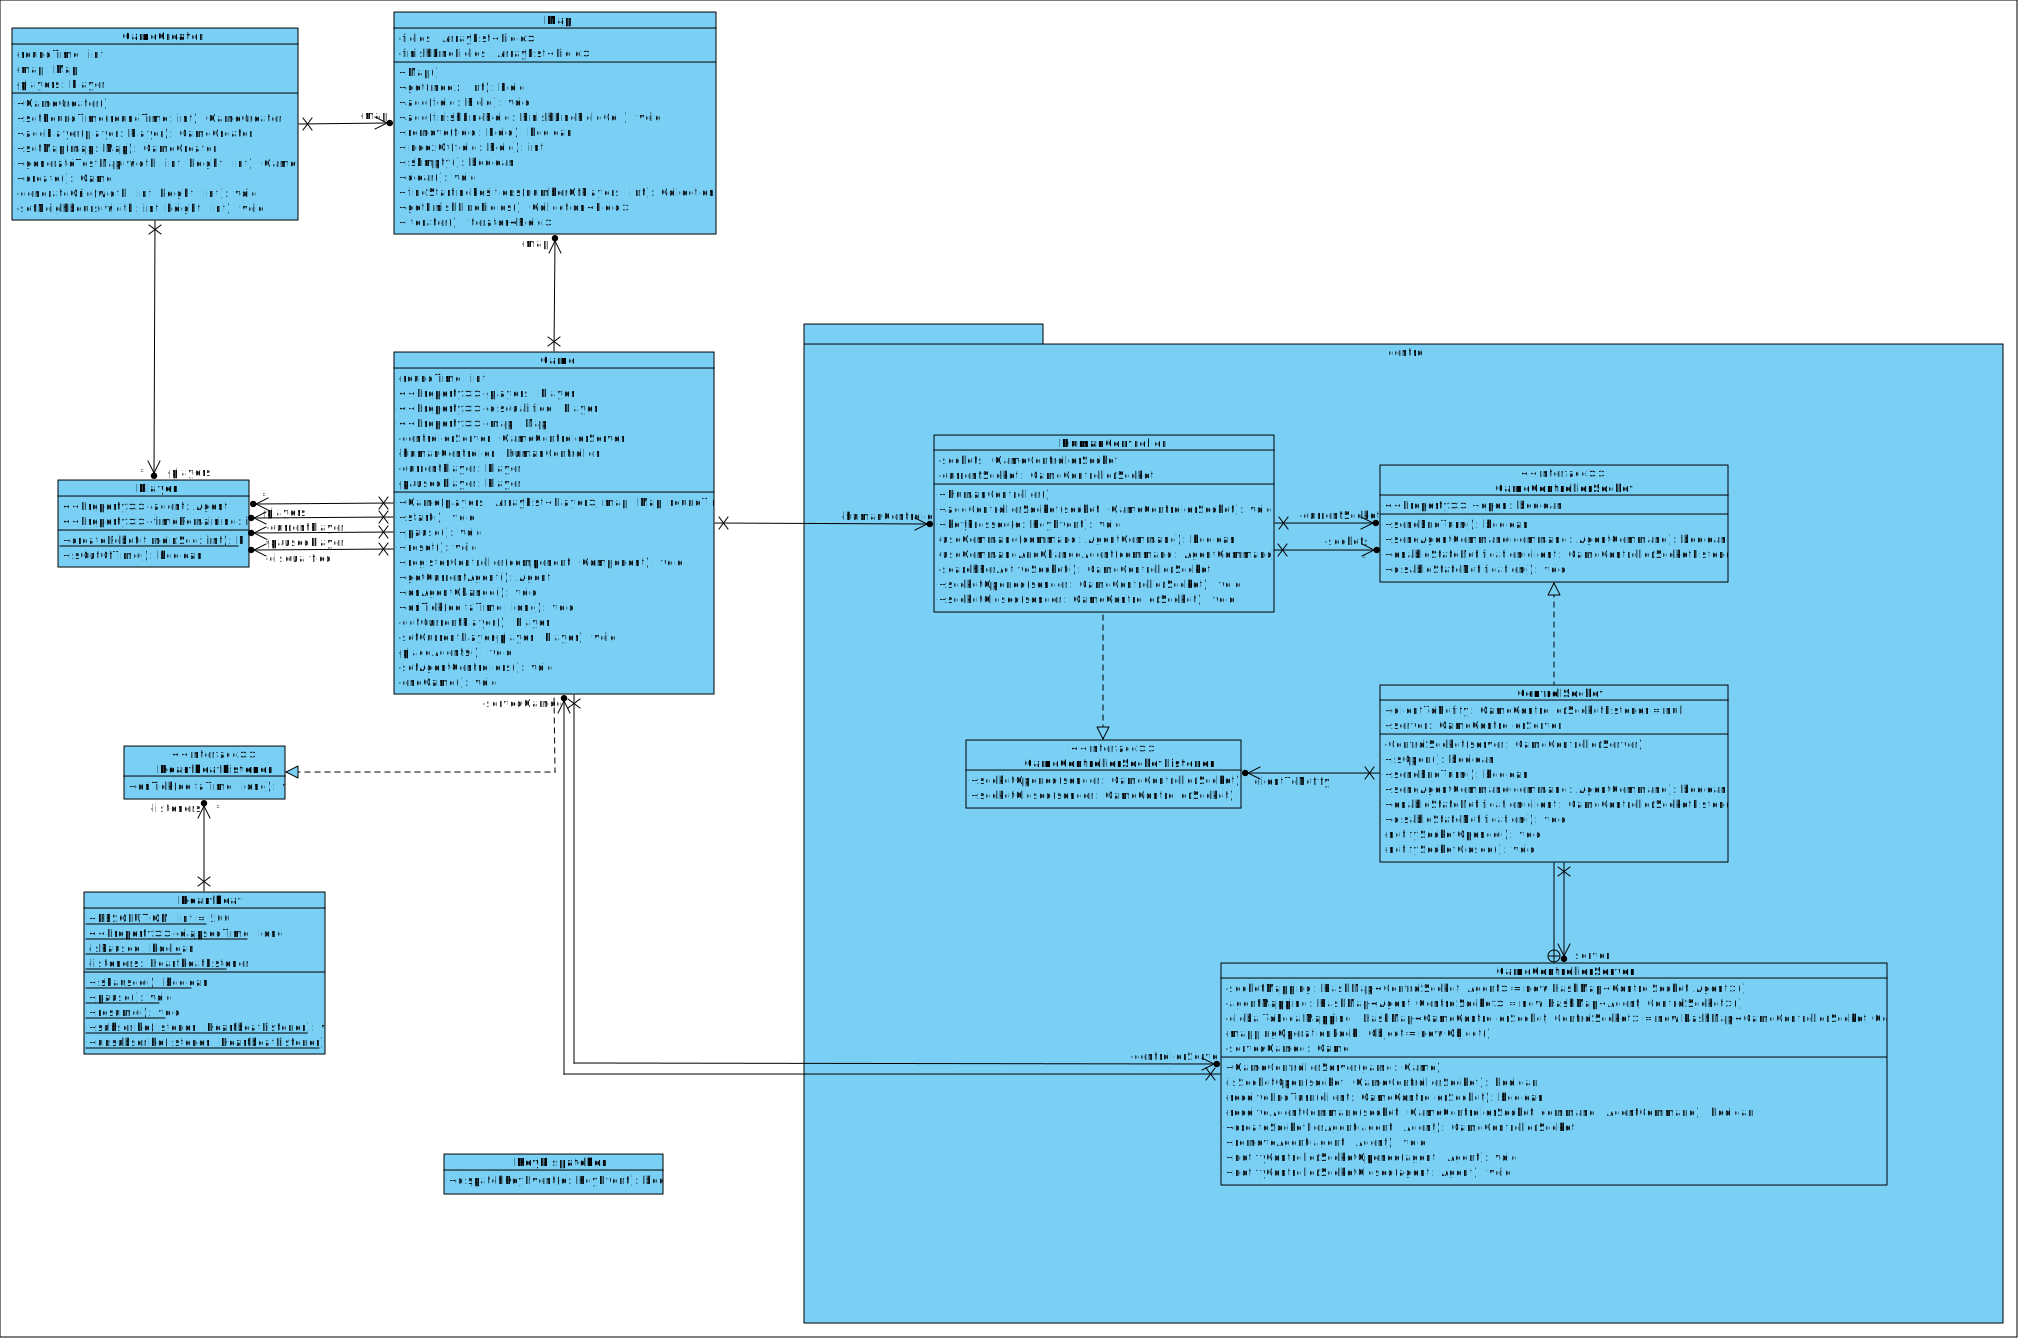
\includegraphics[width=\linewidth]{chapters/chapter07/gamepackage.pdf}
		\caption{Game package osztálydiagram}
		\label{Game package osztálydiagram}
	\end{center}
\end{figure}

\clearpage


\subsection{Szekvenciadiagram módosítások}
\begin{figure}[h]
	\begin{center}
		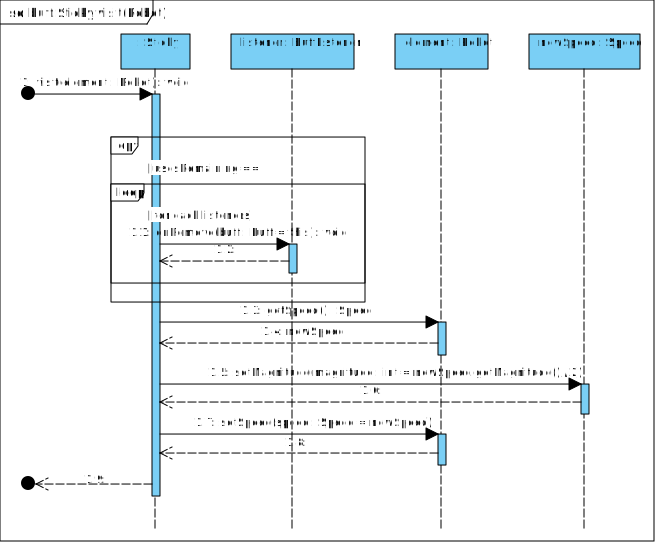
\includegraphics[width=\linewidth]{chapters/chapter07/ragacskopas.pdf}
		\caption{Ragacs kopása}
		\label{Ragacs kopása}
	\end{center}
\end{figure}

\clearpage

\begin{figure}[h]
	\begin{center}
		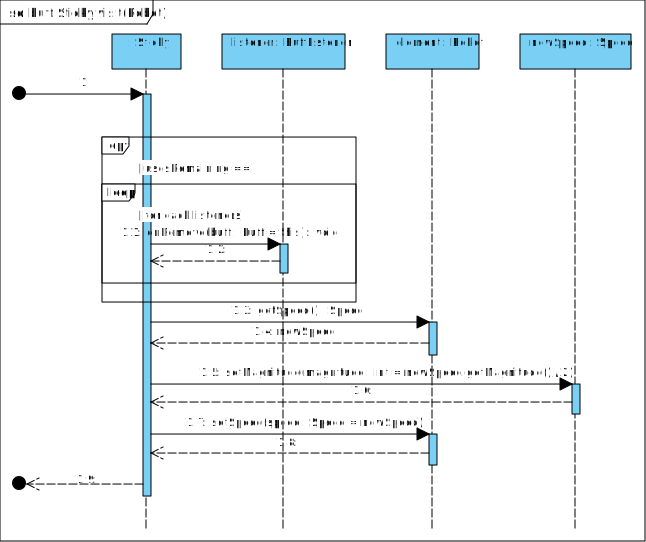
\includegraphics[width=\linewidth]{chapters/chapter07/olajszaradas.pdf}
		\caption{Olaj felszáradása}
		\label{Olaj felszáradása}
	\end{center}
\end{figure}

\clearpage

\begin{figure}[h]
	\begin{center}
		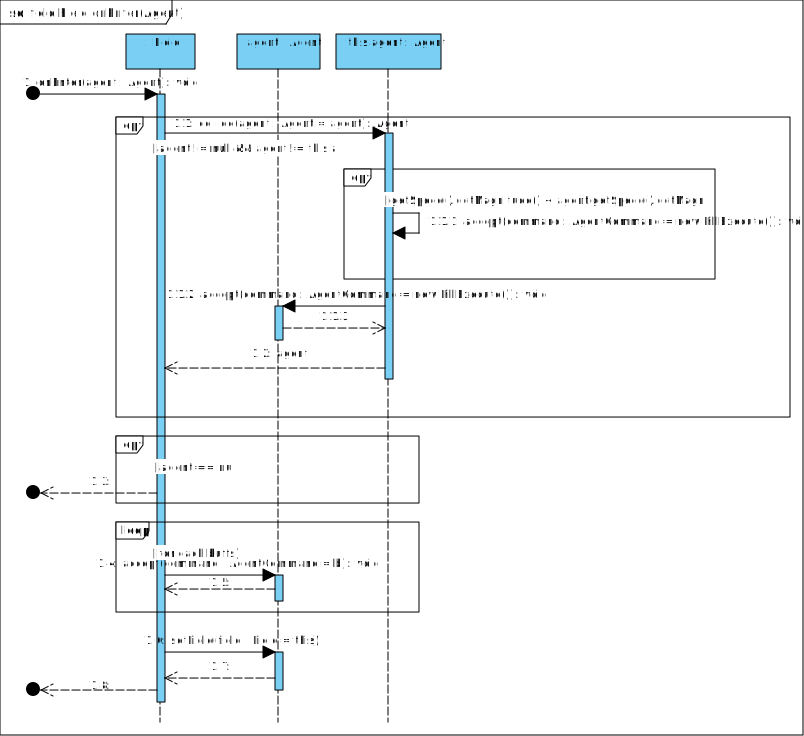
\includegraphics[width=\linewidth]{chapters/chapter07/utkozes.pdf}
		\caption{Robotok ütközése}
		\label{Robotok ütközése}
	\end{center}
\end{figure}

\clearpage


\section{Prototípus interface-definíciója}

\subsection{Az interfész általános leírása}
Az interfész a szabványos bemenetről tud fogadni parancsokat, a kimenetet pedig a szabványos kimenet jelenti. Ennek köszönhetően a használat
leegyszerűsödik, mivel a ki/bemenetek átirányításával lehetőség adódik ki/bemeneti fileokat megadni, melyek lehetőséget adnak a helyes működés
ellenőrzésére, amennyiben összehasonlításra kerülnek egy referenciakimenettel (mely az elvárt működést írja le.). Egy teszteset a prototípusnak
adható parancsok szekvenciájából, kimenet pedig az ezekre adott válaszokból áll. A tesztet sikeresnek mondhatjuk, ha a referenciakimenettel 
megegyező eredményt produkál. \\
A -rng kapcsolóval lehetőség adódik a randomizálható értékek generálására. Ezen kapcsoló hiányában a program tökéletesen determinisztikusan működik,
ez a funkció csak a tesztelői input rövidítésére szolgál. Viszont nem használható automata ellenőrzés esetén.\\
A -log kapcsoló lehetőséget ad a logok szintjének állítására például all/test/debug. \\

\subsection{Bemeneti nyelv}
\comment{Definiálni kell a teszteket leíró nyelvet. Külön figyelmet kell fordítani arra, hogy ha a rendszer véletlen elemeket is tartalmaz, akkor a véletlenszerűség ki-bekapcsolható legyen, és a program determinisztikusan is futtatható legyen. A szálkezelést is tesztelhető, irányítható módon kell megoldani.}

\begin{itemize}
\item Parancs1
	\begin{itemize}
	\item Leírás:
	\item Opciók:
	\end{itemize}
\item Parancs2
	\begin{itemize}
	\item Leírás:
	\item Opciók:
	\end{itemize}

\end{itemize}

\comment{Ha szükséges, meg kell adni a konfigurációs (pl. pályaképet megadó) fájlok nyelvtanát is.}

\subsection{Kimeneti nyelv}
\comment{Egyértelműen definiálni kell, hogy az egyes bemeneti parancsok végrehajtása után előálló állapot milyen formában jelenik meg a szabványos kimeneten.}

\section{Összes részletes use-case}
\comment{A use-case-eknek a részletezettsége feleljen meg a kezelői felületnek, azaz a felület elemeire kell hivatkozniuk.
Alábbi táblázat minden use-case-hez külön-külön.}

\usecase%
{Új játék indítása}%
{Elindíthatunk egy új játékot}%
{Játékos, Játék}%
{A játékosok számának megadása után a Játékos kezdeményezheti a játéknak az elindítását}

\usecase%
{Játékparaméterek megadása}%
{Új játék paramétereinek megadása}%
{Játék}%
{Játékosok megadhatják, hogy hányan vannak, milyen időkorláttal kívánnak játszani}

\usecase%
{Játék megnyerése}%
{Játék végső helyzete alapján győztes eldöntése}%
{Játékos, Játék}%
{Ha minden Játékosnak lejár akkor a megtett út alapján eldől, hogy ki a győztes}

\usecase%
{Játék elvesztése}%
{Játék végső helyzete alapján vesztesek eldöntése}%
{Játékos, Játék}%
{Ha minden Játékosnak lejár akkor a megtett út alapján eldől, hogy kik a vesztesek}

\usecase%
{Játék elmentése}
{A játék jelenlegi állásának fájl(ok)ba mentése}
{Játékos, Játék}
{A Játékos megadja az elérési utat és a Játék elmenti a játékot}

\usecase%
{Játék betöltése}
{A játék fájlból való betöltése}
{Játékos, Játék}
{A Játékos megadja az elérési utat és a Játék betölti a játékot}

\usecase%
{Logolás}
{A játékos meghatározza, hogy logoljon a program}
{Játékos, Játék}
{A Játékos beállítja a logolás mértékét a -log kapcsolóval}

\usecase%
{Randomizálás}
{A játékos meghatározza, hogy véletlenszerű értékekkel működjön a program}
{Játékos, Játék}
{A Játékos az -rng kapcsolóval tudja ezt állítani}


\section{Tesztelési terv}
\comment{A tesztelési tervben definiálni kell, hogy a be- és kimeneti fájlok egybevetésével miként végezhető el a program tesztelése. Meg kell adni teszt forgatókönyveket. Az egyes teszteket elég informálisan, szabad szövegként leírni. Teszt-esetenként egy-öt mondatban. Minden teszthez meg kell adni, hogy mi a célja, a proto mely funkcionalitását, osztályait stb. teszteli. Az alábbi táblázat minden teszt-esethez külön-külön elkészítendő.}

\teszteset{...}{...}{...}

\section{Tesztelést támogató segéd- és fordítóprogramok specifikálása}
A csapat a tesztelést támogató progamot egy egyszerű különbségellenőrzőnek képzeli el, mely képes a kimenetet egy referenciafilelal összehasonlítva megmondani,
hogy az output melyik sorában van eltérés a várt kimenettől. Ennek segítségével lehetőség nyílik a hiba felderítésére és javítására. Bemenetei a program által adott
teszteset outputja és a referenciafile. Kimenete az eltérések. 

